%=================================================================
\section{GPU Testbed and Selected CUDA kernels} \label{sec:methodChar}
Several different benchmarks have been proposed in the literature to measure and assess existing GPGPU heterogeneous architectures, such as Rodinia~\citep{Rodinia:Che:2009}, Parboil~\citep{Stratton:2012:Parboil} and SHOC~\citep{Danalis:2010:SHOC}. Rodinia benchmark was devised for heterogeneous parallel computing research, it has had a high level of acceptance in the community and its applications represent different high-level domains or behaviours,  called the Berkeley dwarfs~\cite{asanovic2009dwarfs}. In this work, we have selected  a set of GPU Applications from the Rodinia Benchmark suite and  other classical algorithms of linear algebra. First to all, we present in the next subsection the different GPUs that we used for our experiments. After in Subsection~\ref{ssec:useCases}, we characterize each one of the kernel that we used for our experiments.

%For each application we iterated over the values of one or two parameters, with some applications invoking the same kernel multiple times on each execution. During our evaluation, all applications were executed using the CUDA profiling tool \textit{nvprof}. Each experiment is presented as the average of ten executions, with a confidence interval of 95\%. In this section we describe the GPU applications, GPU testbed used to do this work.

%---------------------------------------------------------------------------

\subsection{GPU Testbed}\label{ssec:GPUTestbed}
For our experiments in the Chapter~\ref{chap:BSPmodel} and Chapter~\ref{Chap:ML} we used 9 different GPUs, described in Table~\ref{tab:GPUs}, with 5 belonging to Kepler architecture (Compute Capability 3.X), 3 to Maxwell (C.C. 5.X) and 1 to Pascal (C.C. 6.x). More information about these GPUs are presented in Table~\ref{tab:CC} and we have described the main changes of hardware and software between architectures in Section~\ref{ssec:GPUroadmap}. 

%Experiments with the Tesla Pascal P-100 were performed accessing the Free OpenPOWER Cloud by Unicamp, running in an IBM OpenPOWER Server configured with 16 physical cores, up to 128 simultaneous treads or vcpus, and 2 x NVIDIA GPU Tesla-P100, connected via NVLINK 1.0. 

% \todoRaph{You described where the Pascal experiments were performed. And the other boards? \textbf{Corrected - That was question of acknowledge}}

\begin{table}[htpb]
    \centering
    \scalebox{0.75}{
    \begin{tabular}{lccccccc}
        \toprule
        \textbf{Model}&\textbf{C.C.}&\textbf{Memory}&\textbf{Bus}&\textbf{Bandwidth}&\textbf{L2}&\textbf{Cores/SM}&\textbf{Clock} \\ \bottomrule
        GTX-680&3.0&2 GB&256-bit&192.2 GB/s&0.5 M&1536/8&1058 Mhz \\ \midrule 
        Tesla-K40&3.5&12 GB&384-bit&276.5 GB/s&1.5 MB&2880/15&745 Mhz \\ \midrule
        Tesla-K20&3.5&4 GB&320-bit&200 GB/s&1 MB&2496/13&706 MHz\\ \midrule
        %Titan Black&3.5&6 GB&384-bit&336 GB/s&1.5 MB&2880/15 &980 Mhz \\ \midrule
        Titan&3.5&6 GB&384-bit&288.4 GB/s&1.5 MB&2688/14&876 Mhz\\ \midrule
        Quadro K5200&3.5&8 GB&256-bit&192.2 Gb/s&1 MB&2304/12&771 Mhz \\ \midrule
        Titan X&5.2&12 GB&384-bit&336.5 GB/s&3 MB&3072/24&1076 Mhz \\ \midrule
        GTX-970&5.2&4 GB&256-bit&224.3 GB/s&1.75 MB&1664/13&1279 Mhz\\ \midrule
        GTX-980&5.2&4 GB&256-bit&224.3 GB/s&2 MB&2048/16&1216 Mhz \\ \midrule
        Pascal-P100&6.0 GB&16 GB&4096-bit&732 GB/s&4 MB&3584/56&1328 Mhz\\ \midrule
    \end{tabular}}
    \caption{Hardware specifications of the GPUs in the testbed}
    \label{tab:GPUs}
\end{table}

\subsection{Selected CUDA kernels}\label{ssec:useCases}
The  source code for all the use cases, experiments and results are available\footnote{Hosted at GitHub: \texttt{\scriptsize https://github.com/marcosamaris/gpuperfpredict} [Accessed on March 2018]} under Creative Commons Public License for the sake of reproducibility. 

Our benchmark contains 4 different strategies for \emph{matrix multiplication}~\citep{CUDAGuide}, 2 algorithms for \emph{matrix addition}, 1 dot product algorithm, 1 vector addition algorithm and 1 \emph{maximum sub-array problem} algorithm~\citep{Cleber:Thesis}, and 11 CUDA kernel functions belonging to 6 applications from Rodinia benchmarking suite (see Table~\ref{tab:Rodinia}). The remainder of this section discusses some details of these algorithms, and introduces a code of letters for each application, used in Chapter~\ref{chap:BSPmodel} and Chapter~\ref{Chap:ML}.

\subsubsection{Matrix Multiplication}
Matrix multiplication is the core of many scientific areas. This operation is highly used in areas like deep learning, visual computing and digital images processing, among others. The analysis and modeling of these algorithms brings a better understanding and help to researcher and developer of Job Management Systems to deal with this mathematical operations.

In this research, we used four different versions of matrix multiplication, these versions differ in memory access optimizations: global memory with non-coalesced accesses (MMGU); global memory with coalesced accesses (MMGC); shared memory with non-coalesced accesses (MMSU); and shared memory with coalesced accesses (MMSC). This algorithm has a high utilization of the Streaming Processors and it obtains a high throughput of communication in the different levels of memory, L2 cache and L1 cache for small matrices. We have adopted \texttt{block\_size}$^2$ threads per block and defined the number of blocks to be square of \texttt{(N + block\_size-1)/block\_size}, dynamically devised from the size of the problem ($N$) and the block size. Aiming to take advance of coalesced accesses the value of \texttt{block\_size} is equal to 16 in our experiments. In Section~\ref{sec:characterization} is presented an communication analysis of this application with different sizes of threads per block.

The asymptotic computational complexity of a square matrix multiplication of size $N$ is $O(N^3)$ in a sequential algorithm, in a CUDA algorithm this complexity is $O(N)$ using $N\times{}N$ threads. In this algorithm each thread requests $N$ elements from both matrices and perform a dot product with these arrays. This CUDA kernel performs $N$ reads from global memory for each matrix and $N$ arithmetic operations. A single write instruction is performed. shared memory is not used in two versions, MMGU and MMGC. In Figure~\ref{fig:matMulGMUN} is shown the source code of the kernel MMGU, we only changed the data access pattern, to permit coalesced accesses to data in global memory. In Figure \ref{fig:matMulGMUN} line 7 is changed to \texttt{Pvalue += A\_d[i * N + k] * B\_d[k * N + j];} and line 10 is changed to \texttt{C\_d[i * Width + j] = Pvalue;}.

\lstset{emph={[2]__global__}, emphstyle={[2]\color{red}\bf },language=C++, keywordstyle=\color{blue}, numbers=left, showspaces=false,
    showstringspaces=false, tabsize=1, breaklines=false,stringstyle=\color{red}, commentstyle=\color{red}, morecomment=[l][\color{magenta}]{\#}}

\begin{figure}[htpb]
\centering
{\scriptsize
\begin{lstlisting}
__global__ void matMul(float* C_d, float* A_d, float* B_d, int N) {
  float Pvalue = 0.0;
  int j = blockIdx.x * blockDim.x + threadIdx.x;
  int i = blockIdx.y * blockDim.y + threadIdx.y;

  for (int k = 0; k < N; ++k) 
    Pvalue += A_d[j * N + k] * B_d[k * N + i];
  
  C_d[j * N + i] = Pvalue;
}

\end{lstlisting}}
\caption{Kernel in CUDA of matrix multiplication only with global memory and uncoalesced accesses (MMGU).}
\label{fig:matMulGMUN}
\end{figure}

The version MMSU and MMSC use shared memory to load data from global memory and to process them with a lower latency of communication. As shared memory is limited in GPU architectures, the implementations of matrix multiplication with shared memory must be tiled. The concept of tiling in shared memory is graphically described with Figure~\ref{fig:TilingMMSU}, with the matrix multiplication. Tiling is a common strategy to partition data into subset called tiles such that each tile fits into the shared memory. This technique splits our problem domain into phases. The tiled process is executed to guarantee that each thread can access data in shared memory to perform its part of the matrix multiplication. 

In process shown in Figure~\ref{fig:TilingMMSU}, a tile process charges a subset from matrix A and Matrix B in the shared memory of the GPU. A barrier synchronization is used to guarantee that all data was loaded in the shared memory, after the calculations are performed, the barrier synchronization guarantees that the shared memory can be safely overwritten. In this application \texttt{tile\_size=block\_size}, consequently the sizes in bytes of both subsets of the matrices will be \texttt{(tile\_size)$^2 \times$FP\_Bytes}, where \texttt{FP\_Bytes} is the size of the single precision used for the application. 

\begin{figure}[htpb]
	\centering
    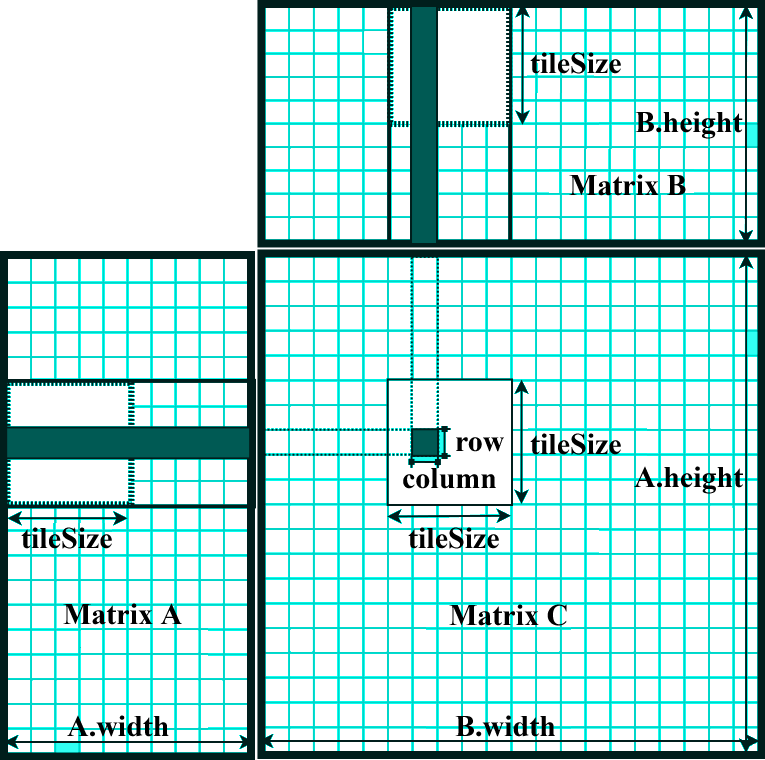
\includegraphics[scale=.3]{images/square-tiling.png}
    \caption{Tiling technique of the Matrix multiplication using shared memory}
    \label{fig:TilingMMSU}
\end{figure}

\subsubsection{Matrix Addition}
For the Matrix addition algorithm, we used two different memory access optimizations: global memory with non-coalesced accesses (MAU); and global memory with coalesced accesses (MAC);  The run-time complexity for a sequential matrix addition algorithm using two matrices of size $N\times{}N$ is $O(N^2)$. In a CUDA implementation, the run-time complexity of the matrix addition is $O(1)$ using $N^2$ threads. In this algorithm each thread request $1$ element from each one of the matrix elements and perform a single addition. The implementation of this kernel is similar than matrix multiplication. In Figure \ref{fig:matMulGMUN} the loop of the line 6-7 is deleted and the statement with the addition is added \texttt{C[tid] = A[tid] + B[tid];}, where \texttt{tid} = \texttt{int tid = i*N + j;}. To take advances of coalesced accesses, \texttt{tid} is changed to \texttt{int tid = j*N + i;}. 

Matrix addition has the same threads hierarchy than matrix multiplication. The blocks are bi-dimensional with \texttt{block\_size}$^2$ threads per block. The size of the grid is square of \texttt{N/block\_size}, dynamically devised from the size of the problem \texttt{N} and \texttt{block\_size}.

\subsubsection{Vector Addition Algorithm (vAdd)}
For two vectors $A$ and $B$, the Vector Addition $C = A + B$ is obtained by adding the corresponding components. In a CUDA implementation, the run-time complexity of the vector addition algorithm is $O(1)$ using N threads, so each threads perform an addition of a position of the vectors $A$ and $B$ and stores the result in the vector $C$. This algorithm is a simplified version of the matrix addition. This application has an uni-dimensional block, the block size used for the experiments is $256$ and the size of the grid is also uni-dimensional and dynamically devised from the size of the problem  \texttt{N} and \texttt{block\_size}. The source code of this kernel is similar than matrix addition, only change the dimension indexes of each threads, i.e. \texttt{int tid = blockDim.x * blockIdx.x + threadIdx.x;}, using only the dimension $x$ of \texttt{blockDim}.

\subsubsection{Dot Product Algorithm (dotP)}
For two vectors $A$ and $B$, the dot product $C = A \cdot B$ is obtained by adding the multiplication of corresponding components of the input, the result of this operation is a scalar. Unlike vector addition, dot product is a reduction from vectors to a scalar. In a GPU algorithm, each thread performs a multiplication of a position of the vectors $A$ and $B$ and stores the result shared variable. Then a reduction using the shared memory is performed and finally a vector with size equal to \texttt{N/block\_size} is transferred to the CPU memory for later processing. The block size used for the experiments is $256$ and the size of the grid is also uni-dimensional and dynamically devised from the size of the problem  \texttt{N} and \texttt{block\_size}.

\subsubsection{Maximum Sub-Array Problem (MSA)}
Let $X$ be a sequence of $N$ integer numbers $(x_1, ... , x_N)$. The Maximum Sub-Array Problem (MSA) consists of finding the contiguous sub-array within $X$ which has the largest sum of elements. The solution for this problem is frequently used in computational biology for gene identification, analysis of sequence of protein and DNAs, identification of hydrophobic regions, among others. The implementation used in this paper creates a kernel with 4096 threads, divided in 32 blocks with 128 threads~\citep{Cleber:Thesis}. The $N$ elements are divided in intervals of $N/t$, and each block receives a portion of the array. The blocks use the shared memory for storing segments, which are read from the global memory using coalesced accesses. Each interval is reduced to a set of 5 integer variables, which are stored in vector of size $5 \times t$ in global memory. This vector is then transferred to the CPU memory for later processing. 

A summary of each one of these applications is shown in Table~\ref{tab:useCases}, in this table is shown the thread hierarchy and the request shared memory per block in each kernel. In column \texttt{dimGrid} and \texttt{dimBlock} is shown how each solution is associated to the dimension of the problem. Column Shared Mem shows the size of shared memory that each kernel needs per block.

\begin{table}[htpb]
    \centering 
    \scalebox{.9}{
        \begin{tabular}{cccccc} 
            \midrule\midrule
            \textbf{Application} & \textbf{Param} & \textbf{Kernel}& \textbf{\texttt{dimGrid}}&  \textbf{\texttt{dimBlock}}&\textbf{Shared Mem}\\\midrule\midrule   
            \multirow{4}{*}{Matrix Mul} & \multirow{4}{*}{1} &MMGU &\multirow{4}{*}{(GS, GS, 1)}&\multirow{4}{*}{ (BS, BS, 1)}&\multirow{4}{*}{($BS^2\times{}2\times{}4B$)}\\      
            &  &MMGC & & &\\
            &  &MMSU & & &\\   
            &  &MMSC & & &\\\midrule     
            \multirow{2}{*}{Matrix Add} & \multirow{2}{*}{1} &MAU &\multirow{2}{*}{(GS, GS, 1)}&\multirow{2}{*}{ (BS, BS, 1)}&\multirow{2}{*}{0}\\ 
            &  &MAC & & & \\\midrule 
            Vector Add&1  &VAdd &(GS, 1, 1) &(BS, 1, 1)& 0 \\\midrule
            Dot Product&1  &dotP &(GS, 1, 1) &(BS, 1, 1) &($BS\times{}4B$)\\\midrule
            Max. Sub Array&1  &MSA & (48, 1, 1) &(128, 1, 1)&($4096\times{}4B$)\\\midrule
        \end{tabular}}
    \caption{Key linear algebra applications used in the experiments}
    \label{tab:useCases} 
\end{table}

\subsubsection{Rodinia Benchmark Suite}
We selected 11 CUDA kernel functions belonging to 6 applications from Rodinia for the benchmarks (Table~\ref{tab:Rodinia}). Some applications invoke the same kernel multiple times on each execution, resulting in the number of collected samples shown in the last column. For each kernel we iterated over the values of one or two parameters, with the number of iterations indicated inside the brackets. For instance, the Hot Spot application has 2 parameters, with the first iterated among 5 values and the second 4 values, for a total of 20 executions in each machine. %In those applications only some part of them can be compute concurrently, above we will explain the performance behavior of each one of the selected Rodinia benchmarks kernels.

\begin{table*}[htpb]
    \centering 
    \scalebox{.8}{
        \begin{tabular}{cccccc} 
            \midrule\midrule
            \textbf{Application} & \textbf{Berkeley Dwarf} & \textbf{Domain}& \textbf{Param.}& \textbf{Kernels} & \textbf{Samples}\\\midrule\midrule   
            \multirow{2}{*}{Back Propagation (BCK)} & \multirow{2}{*}{Unstructured Grid} & \multirow{2}{*}{Pattern Recognition} &\multirow{2}{*}{1 - [57]}&layerforward&\multirow{2}{*}{57}\\
            &  &  & &adjust-weights  \\\midrule      
            \multirow{2}{*}{Gaussian Elimination (GAU)} & \multirow{2}{*}{Dense Linear Algebra} & \multirow{2}{*}{Linear Algebra} &\multirow{2}{*}{1 - [32]}& Fan1&\multirow{2}{*}{34800}  \\             
            &  &  & & Fan2  \\\midrule
            Heart Wall (HWL) & Structured Grid & Medical Imaging &1 - [84]& heartWall&5270 \\\midrule
            Hot Spot (HOT) & Structured Grid & Physics Simulation &2 - [5,4]& calculate-temp&396288 \\\midrule            
            % Hot Spot 3D (H3D) & Structured Grid & Physics Simulation &2 - [3,10]& hotspotOpt1&150150 \\\midrule                     
            %LavaMD (LMD) & N-Body & Molecular Dynamics &1 - [50]& LavaMD&50\\\midrule
            \multirow{3}{*}{LU Decomposition (LUD)} & \multirow{3}{*}{Dense Linear Algebra} & \multirow{3}{*}{Linear Algebra} &\multirow{3}{*}{1 - [32]}&diagonal&8448 \\
            & & &  & perimeter&8416 \\
        &  &  & & internal&8416 \\\midrule            
            \multirow{2}{*}{Needleman-Wunsch (NDL)} & \multirow{2}{*}{Dynamic Programming} & \multirow{2}{*}{Bioinformatics} &\multirow{2}{*}{2 - [16,10]}& needle-1&21760 \\
             &  &  & & needle-2&21600 \\\midrule
            
        \end{tabular}}
    \caption{Rodinia applications used in the experiments}
    \label{tab:Rodinia} 
\end{table*}

\begin{itemize}
    \item {\bf Back Propagation (BCK):}
BCK trains a layered neural network. The application is comprised of two kernels: Forward Phase (BCK-K1), in which the activation are propagated from the input to the output layer, and Backward Phase (BCK-K2), in which the error between the observed and requested values in the output layer is propagated backwards to adjust the weights and bias values. The time complexity of a back-propagation neural network algorithm on a single processor is of $O(W^3)$; where $W$ is the count of weights in the network. In this CUDA implementation both kernels have a complexity $O(log(BS))$ where $BS=16$. Each block has \texttt{BLOCK\_SIZE}$^2$ number of threads. The number of blocks in the grid is \texttt{(N/block\_size} nad it is dynamically calculated from the layer size ($N$) and the block size.

In kernel (BCK-K1), only one thread (with id 0) in the each block load an element of the input layer on the shared memory, after each thread load an element of the weight matrix on the shared memory. Then, the weight matrix is updated with the values of the input layer. Finally a loop reduction is done with a loop of size log2(block\_size). Inside this loop, log2(block\_size) power instructions are done and log2(block\_size) additions over data in the shared memory. Each interval is reduced to a set of \texttt{grid\_size}$\times$\texttt{block\_size} integer variables. This vector is then transferred to the main memory of the host for later processing. In kernel (BCK-K2), shared memory is not used. According to the source code of (BCK-K2), each thread performs O(1) reads and write in the global memory and does different computations over this data.

\item{\bf Gaussian Elimination (GAU):}
GAU solves a linear system $Ax = b$, the application analyzes an $n\times{}n$ matrix and an associated $1 x n$ vector to solve a 
set of equations with $n$ variables and $n$ unknowns. Gaussian Elimination algorithms has a complexity $O(n^3)$. This application compute the results row by row. The algorithm synchronizes between iterations, but the values calculated in each iteration is computed in parallel, see Figure~\ref{fig:GauCode}.

, where $n$ is the size of the matrix elements in both dimensions, i.e. the matrix is $n\times{}n$. 


The application has two different kernels Fan1 and Fan2, which we call (GAU-K1) and (GAU-K2) respectively. (GAU-1) calculate multiplier matrix and (GAU-2) modify the matrix A into LUD. In the experiments, we varied the size of the matrix. 

In this implementation, First kernel GAU-K1, has a uni-dimensionmal block, each block \texttt{block\_size = 512} threads and the number of block is dynamic and computed with the next expression \texttt{(N/block\_size)}. Second kernel has a bi-dimensional block, its dimension is \texttt{block\_size}$^2$ and \texttt{block\_size = 4} in this implementation. The size of the grid also is dynamic depending to size of the problem $N$and the $BS$ (Block size), and it is computed as \texttt{(N/block\_size)}. Both kernel are iterative, it means that the same kernels are invoked multiple times on a single execution of the whole application. Any of these kernel use the shared memory of the streaming processors. 

\lstset{emph={[2]__global__}, emphstyle={[2]\color{red}\bf },language=C++, keywordstyle=\color{blue}, numbers=left, showspaces=false,
    showstringspaces=false, tabsize=1, breaklines=false,stringstyle=\color{red}, commentstyle=\color{red}, morecomment=[l][\color{magenta}]{\#}}

\begin{figure}[htpb]
\centering
{\scriptsize
\begin{lstlisting}
for (t=0; t<(Size-1); t++) {
		Fan1<<<dimGrid1,dimBlock1>>>(m_cuda,a_cuda,Size,t);
		cudaThreadSynchronize();
		Fan2<<<dimGrid2,dimBlock2>>>(m_cuda,a_cuda,b_cuda,Size,t);
		cudaThreadSynchronize();
	}
\end{lstlisting}}
\caption{Kernel in CUDA of matrix multiplication only with global memory and uncoalesced accesses (MMGU).}
\label{fig:GauCode}
\end{figure}

\item {\bf Heart Wall (HWL):}
HWL tracks the movement of a mouse heart over a sequence of 104 609x590 ultrasound images to record response to the stimulus. In the experiments, we varied the number of frames to process. This kernel has two different stages, in the first stage the kernel performs operations on the first frame to detect initial, partial shapes of inner and outer heart walls in the second stage the kernel presents multiple nested loops that process batches of 10 frames and 51 points in each image. This kernel is very complicated to analyze, i.e. this kernel has 1300 codes lines more or less, it uses 8 variables in the shared memory and 44 variables to store all its computations in each streaming multiprocessor, obtaining a low latency in this process. it runs multiple times depending the number of frame to compute. As the number of threads in a block as the number of blocks in a thread ar uni-dimensionals. For all the experiments, this kernels has a \texttt{block\_size}$= 256$ and a \texttt{grid\_size}$ = 51$. For a total of 13056 threads in each one of the executions. This application modeled a set of  ordinary differential equations (ODEs) that are determined by more than 200 parameters. HWL requires the inclusion of some non-parallel computation into the kernel, leading to a slight warp under-utilization.

% \todoRaph{Describe something about the computations performed in the HWL kernel/application.}

\item {\bf HotSpot (HOT):}
HOT is a tool to estimate processor temperature based on an architectural floor plan and simulated power measurements. This application includes the 2D transient thermal simulation kernel which iteratively solves a series of differential equations to determine block temperatures. This kernel has a bi-dimensional grid and block. The dimension of the block is square of \texttt{block\_size} and \texttt{block\_size}$ = 16$. The size of the grid is the square of \texttt{N/block\_size} and it is dynamic depending the size of the problem and the size of the thread block. In the experiments, we varied two parameters: size of the problem and number of iterations. This application has a single kernel. It uses the shared memory.



\item {\bf LU Decomposition (LUD):}
this is a factorization algoritm, where ''LU'' means \emph{lower upper}, LUD is an algorithm to calculate the solutions of a set of linear equations. The LUD kernel decomposes a matrix as the product of a lower triangular matrix and an upper triangular matrix. This benchmark present tree different kernels (LUD-K1, LUD-K2 and LUD-K3). Similarly to the Gaussian Elimination, the matrix size of this experiment was also iterated. First kernel LUD-K1 (named diagonal) has a static size of threads, the size of threads of this kernels always 16. The second kernel LUD-K2 (named perimeter) has a uni-dimensional block the size of thread per block always is \texttt{block\_size}$*2$, the number of block in the grid also is uni-dimensional and it is computed dynamically with the next expression \texttt{(matrix\_dim-i)/block\_size-1}. The third kernel LUD-K3 (named internal) has a block bi-dimensional, this size is the square of \texttt{block\_size} and \texttt{block\_size}$ = 16$, the grid also is bi-dimensional and it is computed with the same expression than the second kernel, \texttt{(matrix\_dim-i)/block\_size-1}.


\item {\bf Needleman-Wunsch (NDL):}
is a nonlinear global optimization method for DNA sequence alignments. The potential pairs of sequences are organized in a 2D matrix. In the first step, the algorithm fills the matrix from top left to bottom right, step-by-step. In the second step, the maximum path is traced backward to deduce the optimal alignment. Needleman-Wunsch has two CUDA kernels, NDL-K1 and NDL-K2. We iterated over the matrix dimension and penalty positive integer parameters. In both kernels each block use $2180$ KB of shared memory. This implementation use a static number of threads per block of 16 and the grid is dynamically computed with this expression $(N-1)/16$. Where $N$ is the size of the input matrix. 


% \lstset{language=C++, keywordstyle=\color{blue}, numbers=left, showspaces=false,
%     showstringspaces=false, tabsize=1, breaklines=false,stringstyle=\color{red}, commentstyle=\color{red}, morecomment=[l][\color{magenta}]{\#}}

% \begin{figure}[htpb]
% 	\centering
%     \lstset{emph={[2]dim3}, 
%             emphstyle={[2]\color{red}\bf},
%             emph={[3]dimGrid, dimBlock},
%             emphstyle={[3]\color{blue}\bf},
%             emphstyle={\bf}, basicstyle={\ttfamily \scriptsize},
%             commentstyle={\em},
%             keywordstyle={\color{blue}\bf},
%             numbers=left,
%             captionpos=b,
%             xleftmargin=1cm}
% 	\begin{lstlisting}[frame=trBL,language=C,linewidth=.92\linewidth]
% for( int i = 1 ; i <= block_width ; i++){
% 		needle_cuda_shared_1<<<dimGrid, dimBlock>>>(referrence_cuda, matrix_cuda
% 		                                      ,max_cols, penalty, i, block_width); 
% 	}
% 	for( int i = block_width - 1  ; i >= 1 ; i--){
% 		dimGrid.x = i;
% 		dimGrid.y = 1;
% 		needle_cuda_shared_2<<<dimGrid, dimBlock>>>(referrence_cuda, matrix_cuda
% 		                                      ,max_cols, penalty, i, block_width); 
% 	}
	
% 	\end{lstlisting}
% \caption{Launched kernel with its respective dimension variables dimBlock and dimGrid}
% \label{fig:dimGridBlock}
% \end{figure}

\end{itemize}
